\section{Models and Algorithms}\label{tes}
%--------------------------------------------------------------------------------------
\subsection{Voronoi Tessellations}\label{tes:sec:vor}
A Voronoi Diagram is a partitioning of a space $S$ by a set of points. Given $n$ points (seed points) the the space, $P = \{p_0,p_2,...,p_{n-1}\}, P \subset S$, is partitioned into $n$ regions, known as Voronoi Regions or Voronoi Cell, where every point, $s \in S_i,0 \leq i \leq n-1$ in a region, $S_i \subset S$, is closest to a single seed point, $p_i \in P$, in terms of the space's distance measurement operation, $d$ (\cite{okabe2009spatial}). An example of a Voronoi Diagram can be seen in Figure \ref{tes:fig:voreg}.
%--------------------------------------------------------------------------------------
\begin{figure}[H]
	\centering
    \label{tes:fig:voreg}
    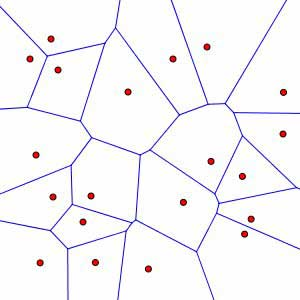
\includegraphics[scale=0.65]{Images/voronoi.jpg}
    \caption{Voronoi Diagram(\cite{voronoipic})}
\end{figure}
%--------------------------------------------------------------------------------------
\subsection{Voronoi Tessellation Generation Algorithms}\label{tes:sec:tga}
%
\subsubsection{Incremental Algorithm}\label{tes:ssec:inc}
The most simplistic of the generation algorithms, the Incremental is an iterative algorithm. Starting from $i=0$ and an empty plane, a seed point, $p_i$ is placed into the plane and TBD (\cite{green1978computing})
%
\subsubsection{Divide and Conquer Algorithm}\label{tes:ssec:dac}
%
\subsubsection{Fortune's Algorithm (Sweep-Line Method)}\label{tes:ssec:fort}
%--------------------------------------------------------------------------------------
\subsection{Clustering Algorithms} \label{tes:sec:clu}
%
\subsubsection{K-Means Algorithm}\label{tes:ssec:kma}
%--------------------------------------------------------------------------------------